\section{Datasets and the Leakage Audit}
\label{sec:audit}

\subsection{Datasets}
We use each dataset's official classes, because the taxonomies conflict across datasets (Section~\ref{sec:filecounts}). Fig.~\ref{fig:gallery} shows random labelled examples, and Table~\ref{tab:audit} summarises the audit.

\begin{itemize}
\item \textbf{WTBD}~\cite{wtbd}: 1{,}065 drone images of six classes (craze, corrosion, surface\_injure, thunderstrike, crack, hide\_craze). It was double-annotated with a reported Cohen's $\kappa=0.897$, and its official split is random (seed 42).
\item \textbf{Wind Surface Defect}~\cite{gfdyolox}, used by BladeYOLO: 3{,}570 files in our public copy against the 3{,}790 the BladeYOLO paper reports. Five classes: corrosion, dirt, hide\_craze, surface\_eye, thunderstrike.
\item \textbf{WTBlade-Defect} (fengChe)~\cite{fengche}, used by BladeYOLO: 10{,}660 Roboflow-exported frames of seven classes (burn, crack, deformity, dirt, oil, peeling, rust).
\item \textbf{Auxiliary sources} used only for the leave-one-dataset-out pools and the audit: WTBs2025~\cite{wtbs2025}, two Beijing Roboflow exports, the DTU NordTank imagery~\cite{dtudata} and drone-footage tiles~\cite{foster}.
\end{itemize}

\begin{figure*}[!t]
\centering
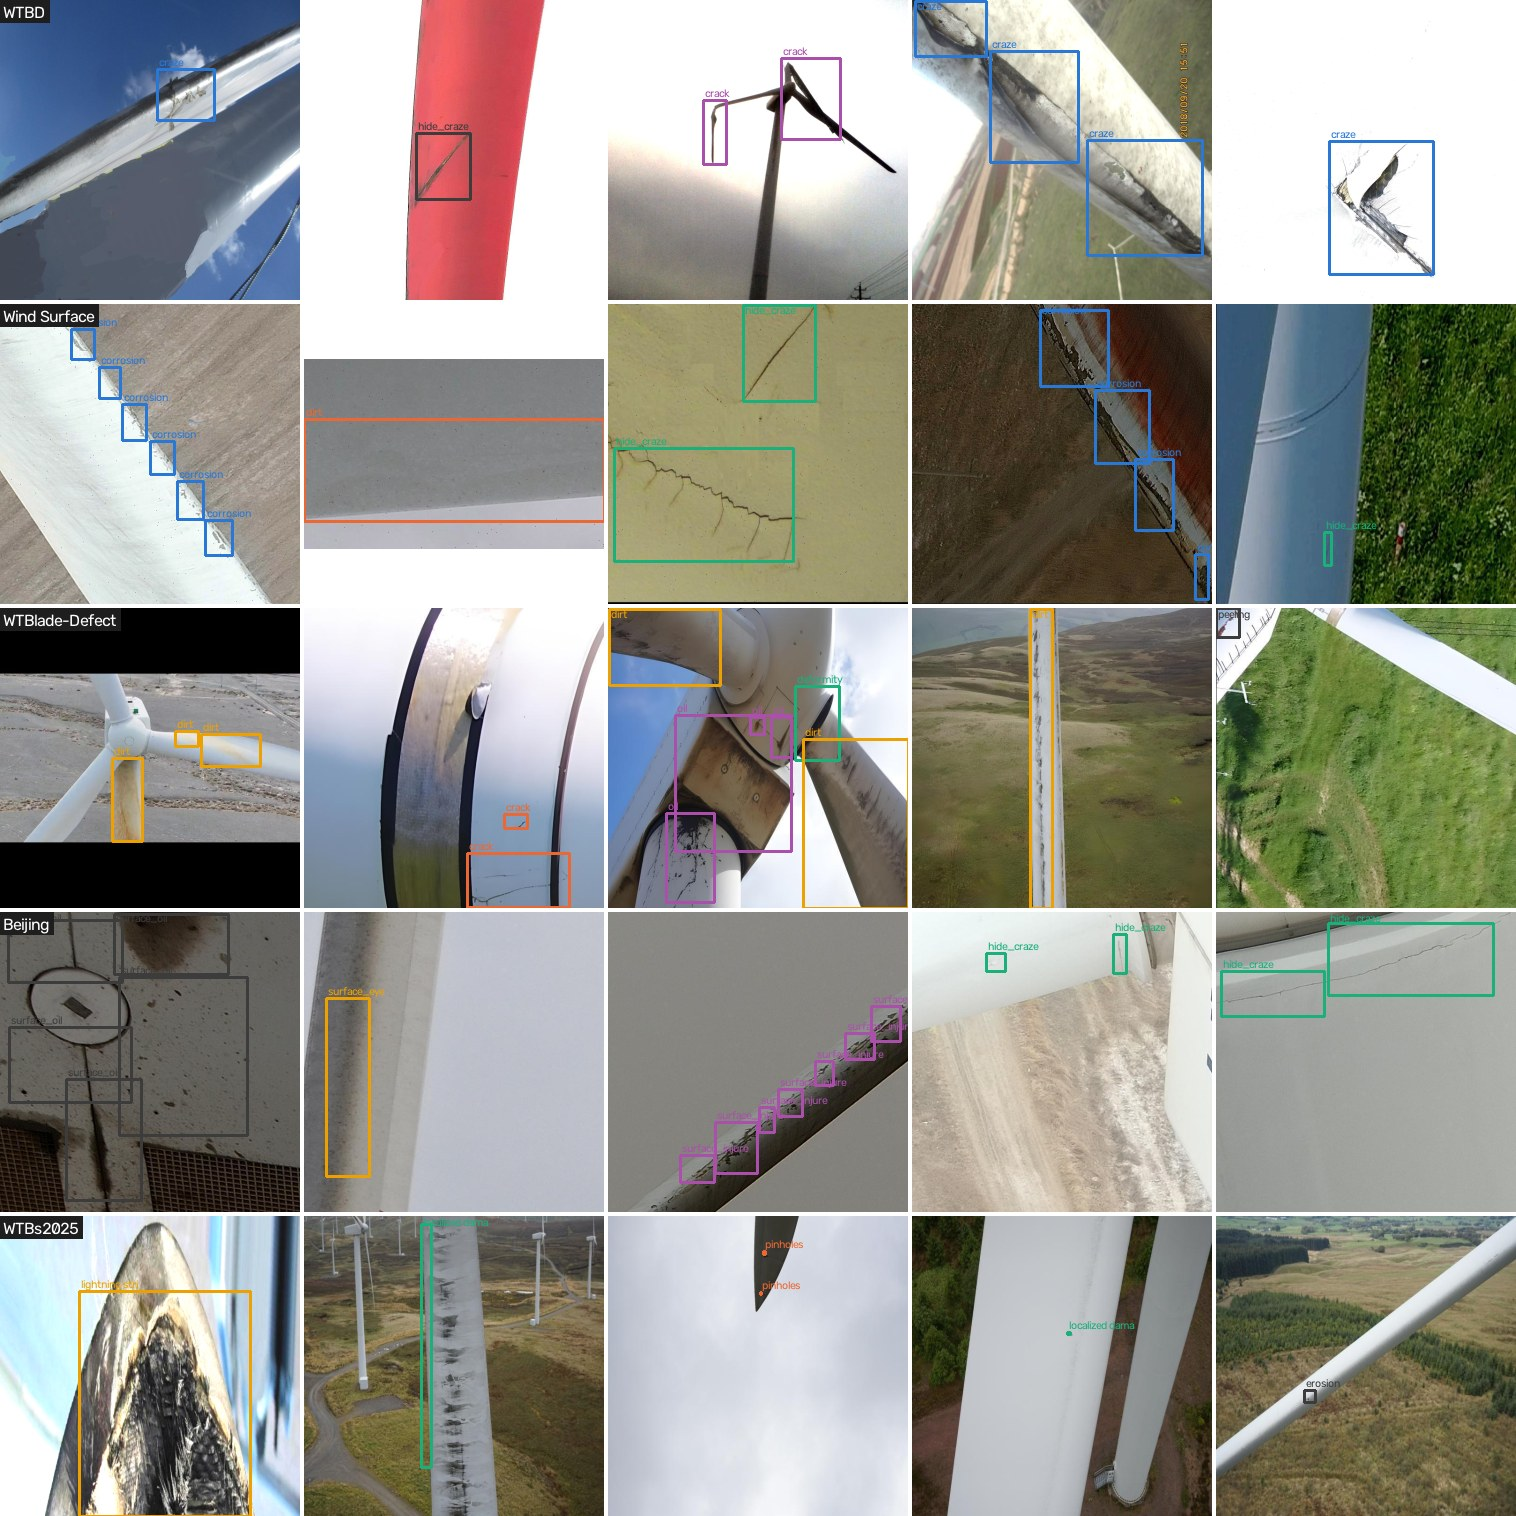
\includegraphics[width=0.86\textwidth]{fig8_dataset_gallery}
\caption{Random labelled training images from each dataset (fixed seed; the first three in each row are required to show a class not yet shown). Colour marks the class within a row. Note the differences in viewpoint and box style, from close-ups with one box (WTBD) to chains of small boxes along an edge (Wind Surface, Beijing) and very small boxes (WTBs2025). Black squares in WTBlade-Defect are the Roboflow export's offline cutout augmentation.}
\label{fig:gallery}
\end{figure*}

\begin{table*}[!t]
\centering
\caption{The three benchmarks and their official splits. Unique images and scenes come from the content-based audit. A \emph{twin} is a near-copy or same-scene image among the images the run trained on.}
\label{tab:audit}
\footnotesize
\begin{tabularx}{\textwidth}{@{}p{0.11\textwidth} r r r p{0.12\textwidth} p{0.2\textwidth} X@{}}
\toprule
Dataset & Files & Unique & Scenes & Official split (train/val/test) & Test images with a training twin & How the twin arises \\
\midrule
WTBD~\cite{wtbd} & 1{,}065 & 597 & $\sim$550 & 745/159/161 & \textbf{125/161 (78\%)} & Duplicate and augmented copies of one photograph, split at random (seed 42) \\
Wind Surface~\cite{gfdyolox} & 3{,}570 & 954 & \textbf{81} & 2{,}856/714 (val\,=\,test) & \textbf{600/714 (84\%)} pixel twins ($r\geq0.99$) & 1{,}785 originals plus one augmented copy each (550 pairs split across train and val); up to 44 tiles per drone photograph (386 of 882 photographs on both sides) \\
WTBlade-Defect~\cite{fengche} & 10{,}660 & 1{,}146 & 803 & 9{,}010/1{,}097/553 & \textbf{499/542 (92\%)} same scene; \textbf{360 (66\%)} copies of a training frame & About three Roboflow augmentation copies per source frame; consecutive drone-video frames \\
\bottomrule
\end{tabularx}
\end{table*}

\subsection{Audit Method}
Files cannot be compared by name or hash, because the copies are flipped, rotated, recoloured or re-encoded. We therefore combine five signals (Algorithm~\ref{alg:audit}):
\begin{enumerate}
\item \textbf{Retrieval:} DINOv2~\cite{dinov2} image embeddings and cosine nearest neighbours.
\item \textbf{Geometric verification:} flip-aware ORB~\cite{orb} keypoint matching with a RANSAC~\cite{ransac} similarity transform; a pair is verified with at least 25 inliers.
\item \textbf{Pixel twins:} the maximum Pearson correlation at $48\times48$ px over the eight flips and quarter-turn rotations; a twin has $r\geq 0.99$.
\item \textbf{Provenance from file names:} Roboflow source prefixes, \texttt{DJI\_xxxx\_r\_c} tile coordinates, and \texttt{\_0}/\texttt{\_1} augmentation pairs.
\item \textbf{Grouping:} union-find over all of the above, with DINOv2 cosine $\geq 0.93$ counted as the same scene. Deduplication is non-chaining, so that a chain of weak matches cannot merge unrelated images.
\end{enumerate}

\begin{algorithm}[!t]
\caption{Content-based twin and scene audit}
\label{alg:audit}
\footnotesize
\begin{algorithmic}[1]
\Require images $\mathcal{I}$, file names, thresholds $\tau_{\cos}=0.93$, $n_{\mathrm{inl}}=25$, $\tau_{r}=0.99$
\State $e_i \gets \mathrm{DINOv2}(i)/\lVert\cdot\rVert$ for all $i\in\mathcal{I}$
\State $\mathcal{U} \gets$ union-find over $\mathcal{I}$
\For{each $i$ and its $k$ nearest neighbours $j$ by $e_i^\top e_j$}
  \If{$e_i^\top e_j \geq \tau_{\cos}$} \textsc{Union}$(i,j)$ \Comment{same scene}
  \EndIf
  \If{$\max_{g\in D_4}\#\mathrm{inliers}(\mathrm{ORB}(i), \mathrm{ORB}(g(j))) \geq n_{\mathrm{inl}}$} \textsc{Union}$(i,j)$
  \EndIf
  \If{$\max_{g\in D_4} r(i_{48}, g(j)_{48}) \geq \tau_r$} \textsc{Union}$(i,j)$; mark pixel twin
  \EndIf
\EndFor
\State \textsc{Union} images sharing a source prefix, a parent photograph (tile name) or an \texttt{\_0}/\texttt{\_1} stem
\State flag test image $t$ as \emph{leaked} if its group contains an image the run trained on
\State \Return groups (scenes), per-image flags
\end{algorithmic}
\end{algorithm}

Example sheets were checked by eye for every dataset and every outcome. On Wind Surface, the first pixel comparison (flips only) found 532 of 714 validation images (75\%). Adding rotations and restricting the comparison to the images actually trained on gives 600 (84\%). The Wind Surface ``no-twin'' subset has no near-identical copy in training. Most of it, however, comes from drone photographs with other tiles in training, so it is cleaner rather than leak-free. Fig.~\ref{fig:twins} shows test images and their training twins, drawn at random.

\begin{figure*}[!t]
\centering
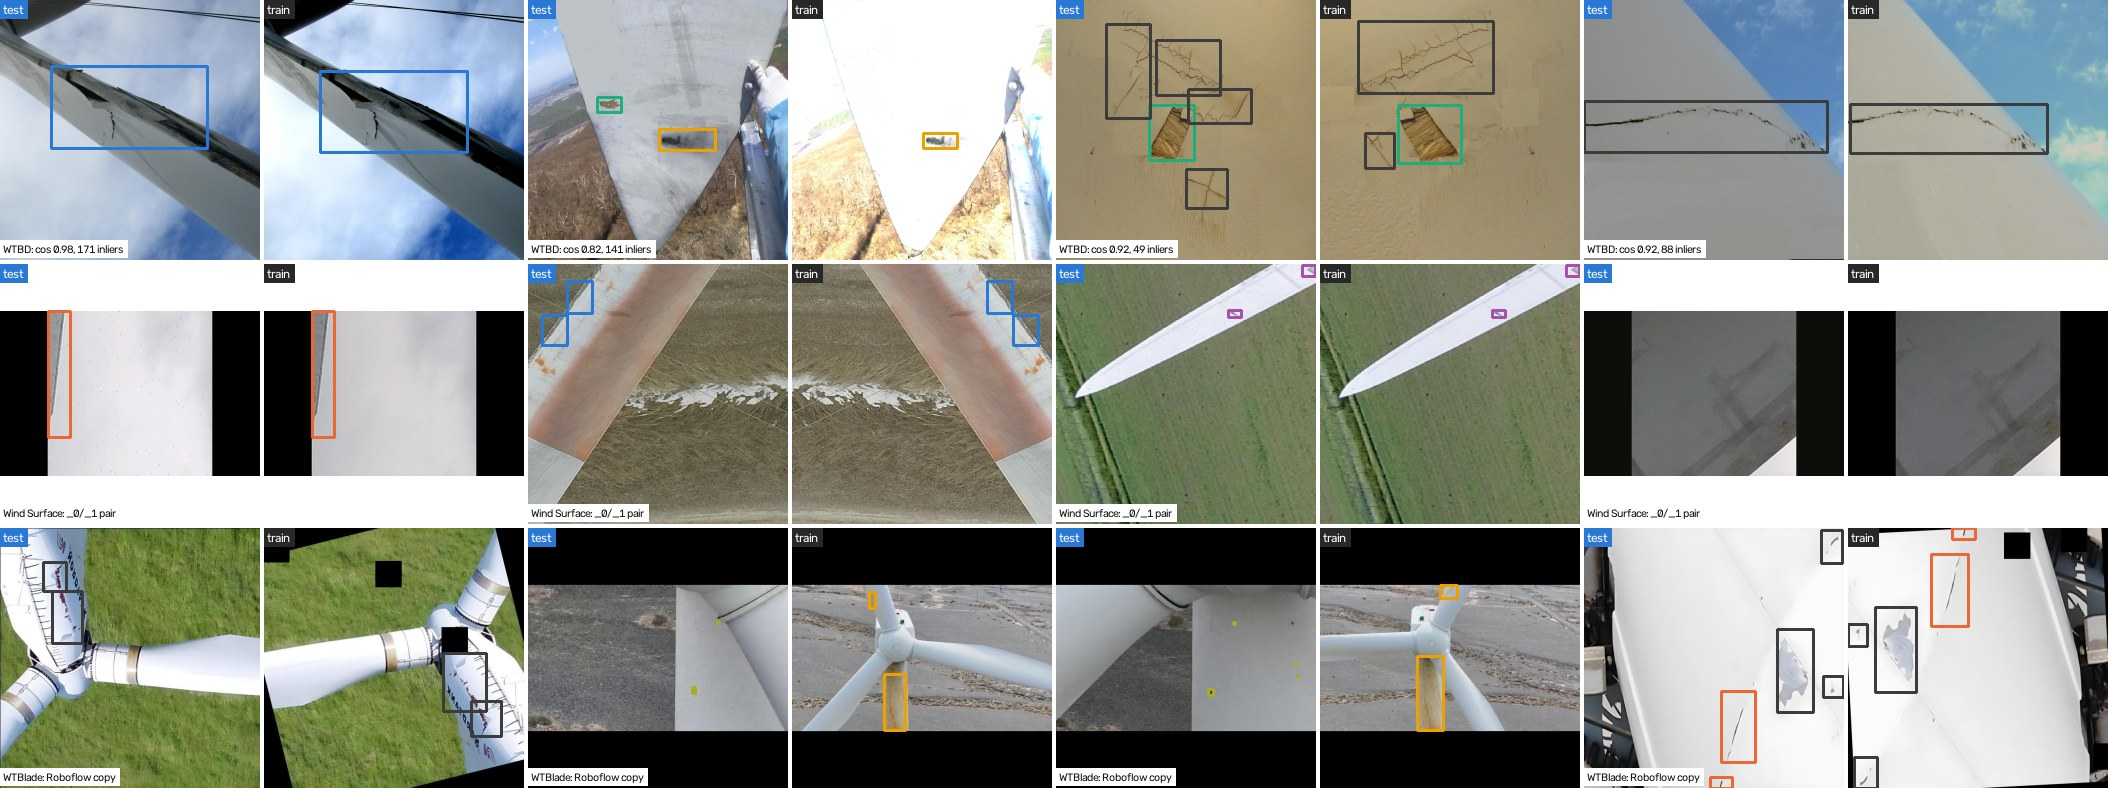
\includegraphics[width=\textwidth]{fig10_twins}
\caption{Official test images (blue tag) next to their training twins (black tag), drawn at random with a fixed seed from the leaked subsets. Labels are drawn as supplied. Row 1: WTBD, with DINOv2 cosine and ORB inliers. Row 2: Wind Surface \texttt{\_0}/\texttt{\_1} pairs split across the partition. Row 3: WTBlade-Defect Roboflow copies of one source frame.}
\label{fig:twins}
\end{figure*}

\subsection{What the File Counts Hide}
\label{sec:filecounts}
File count is a poor guide to the information a dataset holds (Fig.~\ref{fig:size}). Wind Surface's 3{,}570 files come from about 81 independent scenes. All its \texttt{surface\_eye} boxes (412 in the raw files, 103 after deduplication) come from tiles of a single photograph. Any \texttt{surface\_eye} score on the original split, including published ones, was therefore measured on tiles of a training photograph. WTBD has far fewer files and far more independent scenes per class. Three more findings limit what can be merged:
\begin{itemize}
\item \textbf{Same-named classes do not match across datasets.} Mutual crop retrieval between same-named classes is at most 0.33, apart from the two Beijing exports, which are the same data.
\item \textbf{Datasets overlap under other names.} WTBs2025 shares 1{,}499 images with WTBlade-Defect under different class names (peeling becomes erosion). The Beijing exports contain WTBD test photographs.
\item \textbf{Licences are not what the export pages say.} ``NORDTANK'' is legible on many WTBlade-Defect nacelles, so the set contains DTU imagery~\cite{shihavuddin,dtudata}, which is CC BY-NC, while its Roboflow page states CC BY 4.0. It also contains synthetic copy-paste images.
\end{itemize}

\begin{figure}[!t]
\centering
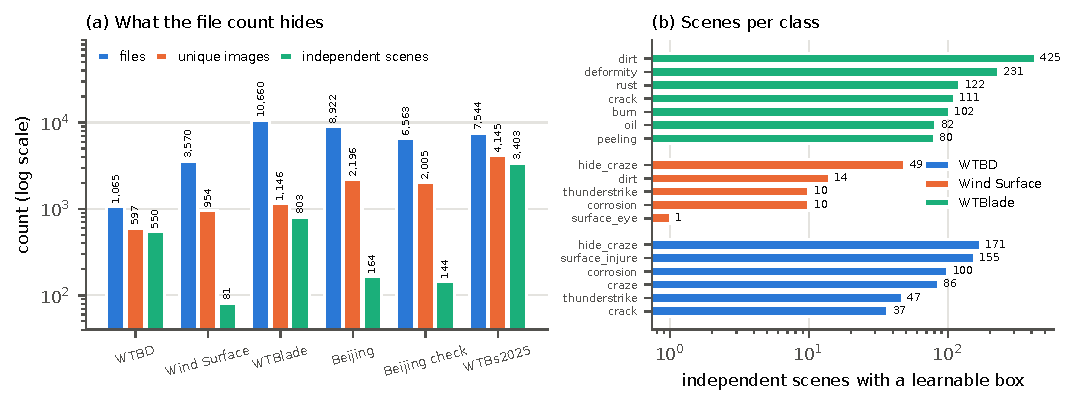
\includegraphics[width=\linewidth]{fig9_effective_size}
\caption{Effective dataset size. (a) Files, unique images and independent scenes per dataset. (b) Independent scenes with a learnable box, per class. A single scene supports Wind Surface's \texttt{surface\_eye}.}
\label{fig:size}
\end{figure}

\subsection{Protocols of Published Work}
The augment-then-split pattern is not specific to one paper (Table~\ref{tab:protocols}). KGP-YOLO expands 130 DTU images to 780 and then splits them 624/78/78~\cite{kgpyolo}. GA-YOLOv5 adds CLAHE copies and uses a random 60/40 split of repeated shots of one turbine~\cite{gayolo}. BladeYOLO's WTBlade numbers use its authors' own 9:1 re-split of 5{,}326 images, which is not public~\cite{bladeyolo}.

\begin{table}[!t]
\centering
\caption{Evaluation protocols of published blade-defect detectors, as read from the papers.}
\label{tab:protocols}
\footnotesize
\begin{tabularx}{\linewidth}{@{}l X@{}}
\toprule
Work & Protocol \\
\midrule
GFD-YOLOX~\cite{gfdyolox} & Wind Surface: 1{,}785 originals plus augmented copies, random split; tiles of one photograph on both sides \\
BladeYOLO~\cite{bladeyolo} & Wind Surface random 4:1 (3{,}790 images, no list); WTBlade 9:1 re-split of 5{,}326 images (not public); no separate validation set; random label fractions \\
KGP-YOLO~\cite{kgpyolo} & Augment (flips, brightness, saturation) before the split; DTU 130 $\rightarrow$ 780 images, 624/78/78; single runs \\
GA-YOLOv5~\cite{gayolo} & 432 DTU images doubled by CLAHE, random 60/40 split of repeated shots of one turbine; best synthetic amount read off the test set \\
WTBD~\cite{wtbd} & Random split, seed 42; no detection baselines \\
\bottomrule
\end{tabularx}
\end{table}
